\chapter{ثوابت التوازن وانزياحاته}\label{ch:b2:equilibrium-shifts}

يشغّل مصنع الأمونيا مفاعله المحوِّل عند نحو \qty{450}{\celsius} 
و\qty{200}{bar}. في درجة حرارة الغرفة يميل توازن \ce{N2 + 3H2 <=>
2NH3} نحو الأمونيا ميلًا شديدًا بحيث يمكن من حيث المبدأ تحويل خليط من
العنصرين تحويلًا شبه تام؛ ومع ذلك يسخّنه المهندسون، وهو ما يرد التوازن
إلى الوراء، ثم يضغطونه حتى مئتي ضغط جوي، وهو ما يكلّف طاقة كبيرة. والسبب
تسوية بين المدى الذي يمكن أن يبلغه التفاعل والسرعة التي يجري بها. يحوّل
هذا الفصل \omterm{def:b2:reaction-free-energy:gibbs-energy}{طاقة جيبس} في الفصلين السابقين إلى ثابت التوازن في مجلد السنة
الأولى، ويبيّن كيف يتغير هذا الثابت مع درجة الحرارة، ويعدّ الشروط التي
يمكن للمجرّب أن يختارها بحرية، ويتنبأ بالاتجاه الذي ينزاح فيه التوازن حين
تتغير درجة الحرارة أو الضغط أو التركيب.

\begin{recall}
\Cref{ch:b2:reaction-free-energy}: محك التطور $\Delta_r G\,\dd\xi
\leq 0$ وعلاقة جيبس--هلمهولتز؛
و\cref{ch:b2:chemical-potential}: $\Delta_r G = \Delta_r G^\circ + RT\ln Q$.
ومجلد السنة الأولى: خارج التفاعل $Q = \prod_i a_i^{\nu_i}$، وثابت التوازن
القياسي $K^\circ$ بوصفه قيمة $Q$ عند التوازن، وقانون فعل الكتلة والقاعدة
«$Q < K^\circ$: في الاتجاه المباشر»، وكلها مذكورة هناك بوصفها قوانين؛
وجداول التقدم؛ والحالات النهائية لتفاعل واحد أو لتفاعلين. وقد وعد أيضًا
بأن يُفسَّر هنا اختيار درجة الحرارة والضغط في صناعة الأمونيا وثالث أكسيد
الكبريت.
\end{recall}

\begin{omfigure}
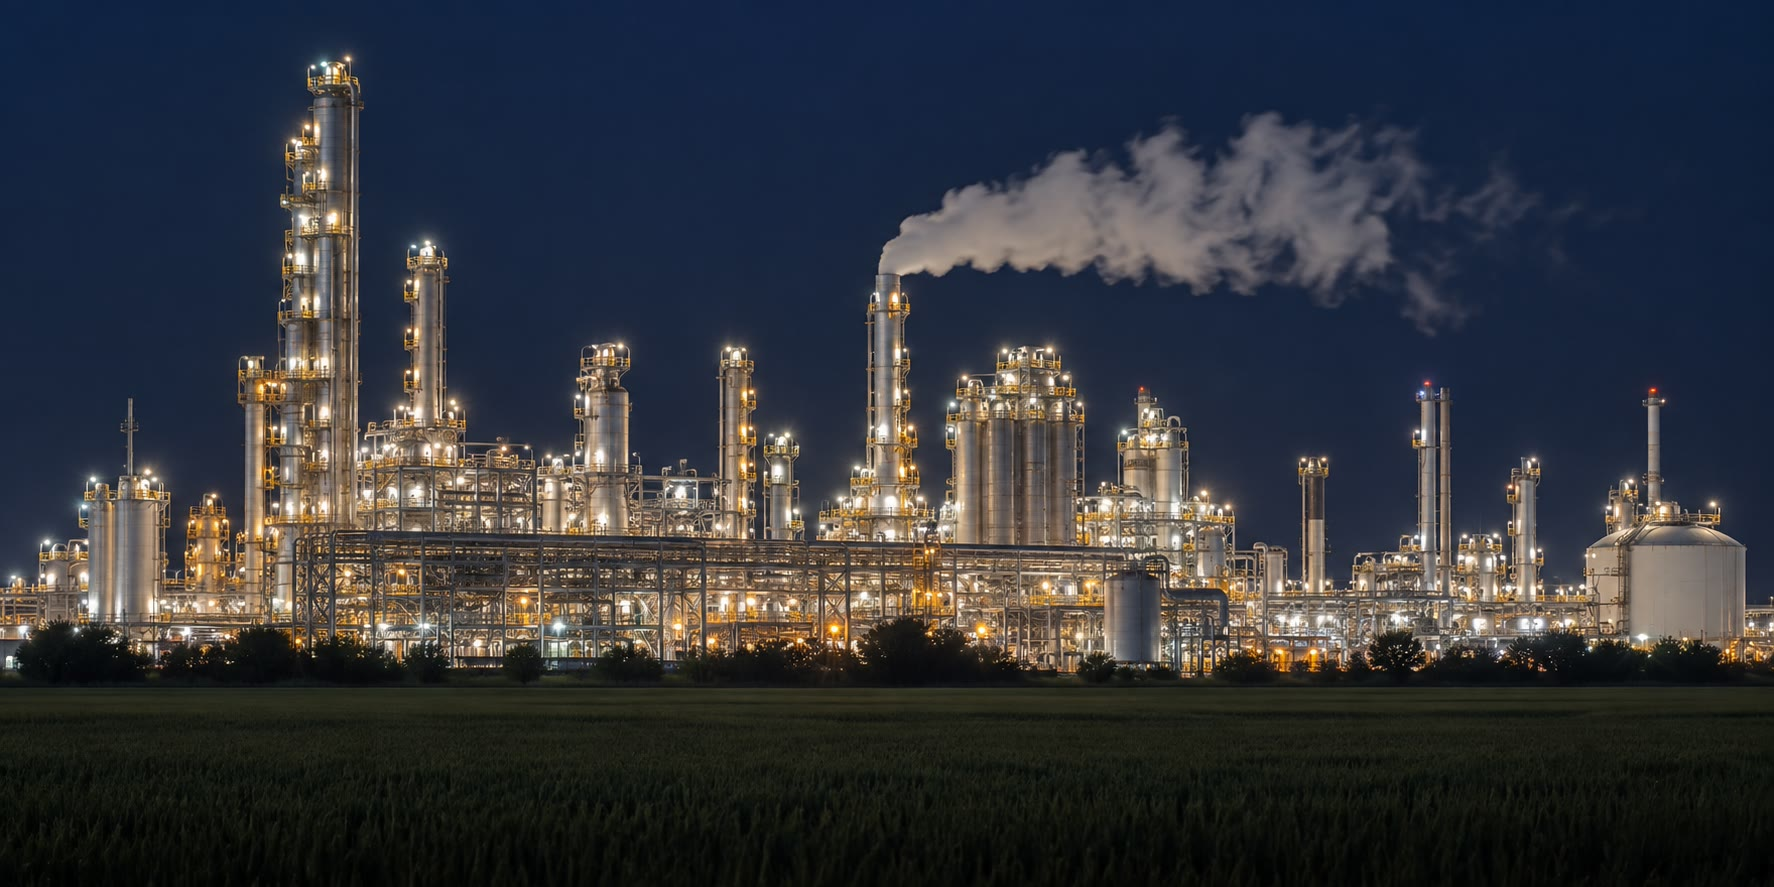
\includegraphics[width=0.7\linewidth]{images/book3/ai/b2-04-ammonia-plant.jpg}

{\small مصنع أمونيا في الليل. في مفاعله المحوِّل يمر النيتروجين والهيدروجين
على حفاز من الحديد عند بضع مئات من الدرجات وبضع مئات من البار؛ واختيار
هذه الشروط هو موضوع مسألة نهاية الأسبوع.}
\end{omfigure}

\section{ثابت التوازن انطلاقًا من طاقة جيبس}

\begin{theorem}[ثابت التوازن القياسي]\label{thm:b2:equilibrium-shifts:k-from-g}
عند التوازن يكون $\Delta_r G = 0$، ويأخذ خارج التفاعل القيمة
\[
  K^\circ(T) = \exp\!\left(-\frac{\Delta_r G^\circ(T)}{RT}\right), \qquad
  \Delta_r G^\circ(T) = -RT\ln K^\circ(T) .
\]
وهو لا يتعلق إلا بدرجة الحرارة.
\end{theorem}

\begin{proof}
يجعل محك التطور الشرطَ $\Delta_r G = 0$ شرطَ التوازن.
ومع $\Delta_r G = \Delta_r G^\circ + RT\ln Q$
(\cref{prop:b2:chemical-potential:delta-g-q})، يعني التوازن أن $\ln Q_{\text{توازن}}
= -\Delta_r G^\circ/(RT)$، وهي دالة في $T$ وحدها لأن $\Delta_r G^\circ$ كذلك.
\end{proof}

\begin{corollary}[قوانين مجلد السنة الأولى]\label{cor:b2:equilibrium-shifts:mass-action}
$\Delta_r G = RT\ln(Q/K^\circ)$. ومنه فالنظام الذي فيه $Q < K^\circ$ يتطور
في الاتجاه المباشر، والذي فيه $Q > K^\circ$ في الاتجاه المعاكس، والذي فيه $Q = K^\circ$ في
توازن (قانون فعل الكتلة).
\end{corollary}

\begin{proof}
نعوّض $\Delta_r G^\circ = -RT\ln K^\circ$ في $\Delta_r G = \Delta_r G^\circ
+ RT\ln Q$؛ فإشارة $\Delta_r G$ هي إشارة $\ln(Q/K^\circ)$، ويتطلب
محك التطور أن يكون $\Delta_r G\,\dd\xi \leq 0$.
\end{proof}

\begin{example}[ثلاثة ثوابت عند \qty{298}{K}]\label{ex:b2:equilibrium-shifts:constants}
تخليق الأمونيا، $\Delta_r G^\circ = \qty{-32.8}{kJ/mol}$: $K^\circ =
\exp(32\,800/(8.314 \times 298.15)) = \num{5.6e5}$ (وتعطي الجداول، بأرقام
أكثر، \num{5.4e5}). وتفكك \ce{N2O4}، $\Delta_r G^\circ =
\qty{+4.7}{kJ/mol}$: $K^\circ = 0.15$. وتفكك الحجر الجيري،
$\Delta_r G^\circ = \qty{+130.4}{kJ/mol}$: $K^\circ = \num{1.5e-23}$، فضغط
التوازن لثنائي أكسيد الكربون فوق الحجر الجيري في درجة حرارة الغرفة
هو $\num{1.5e-23}$ بار، أي لا شيء البتة. وتغيّر قدره \qty{5.7}{kJ/mol} في
$\Delta_r G^\circ$ عند \qty{298}{K} يضرب $K^\circ$ في عشرة أو يقسمه عليها.
% ledger: dfh:NH3_g, s0:NH3_g, janafG:NH3.298.15 (computed in figdata/bachelor-2/thermo-data.py and vant-hoff.py)
\end{example}

تُظهر \omterm{def:b2:reaction-free-energy:gibbs-energy}{طاقة جيبس} للنظام كله الأمر نفسه على هيئة تضاريس: فهي في أدناها عند
تقدم التوازن، حيث ينعدم ميلها، $\Delta_r G$.

\begin{omfigure}
\begin{tikzpicture}
\begin{axis}[
  width=0.7\linewidth, height=5.6cm, xmin=0, xmax=1, ymin=-2.2, ymax=5.2,
  axis x line=bottom, axis y line=left, xlabel={\foreignlanguage{arabic}{التقدم $\xi$ \babelsublr{(mol)}}},
  ylabel={\babelsublr{$G(\xi) - G(0)$ (\unit{kJ})}},
  tick label style={font=\small}, label style={font=\small}, clip=false]
\addplot[omDef, very thick] table[x=xi, y=G] {figdata/out/bachelor-2-gibbs-extent.dat};
\draw[dotted] (axis cs:0.189,-2.2) -- (axis cs:0.189,-0.949);
\fill[omThm] (axis cs:0.189,-0.949) circle (1.6pt);
\node[omThm, anchor=west, font=\small] at (axis cs:0.21,-1.75) {\foreignlanguage{arabic}{التوازن، $\xi = 0.189$}};
\draw[dashed, gray] (axis cs:0,0) -- (axis cs:1,4.728);
\node[gray, font=\scriptsize, anchor=south east] at (axis cs:1,4.75) {$\xi\,\Delta_r G^\circ$};
\end{axis}
\end{tikzpicture}

{\small \omterm{def:b2:reaction-free-energy:gibbs-energy}{طاقة جيبس} لنظام مغلق من الغازات المثالية عند \qty{298}{K} 
و\qty{1}{bar}، انطلاقًا من \qty{1}{mol} من \ce{N2O4}، بدلالة تقدم
\ce{N2O4 <=> 2NO2}. ومع أن $\Delta_r G^\circ > 0$ (الخط المتقطع، الأنواع
النقية)، فإن مزج الغازين يخفض $G$، وتقع القيمة الدنيا عند $\xi =
0.189$، حيث $Q = K^\circ = 0.15$. وعلى يسارها يكون الميل $\Delta_r G =
\partial G/\partial\xi$ سالبًا، وعلى يمينها موجبًا.}
% ledger: dfh:N2O4_g, s0:N2O4_g, dfh:NO2_g, s0:NO2_g (computed in figdata/bachelor-2/gibbs-extent.py)
\end{omfigure}

\section{درجة الحرارة: معادلة فانت هوف}

\begin{theorem}[معادلة فانت هوف]\label{thm:b2:equilibrium-shifts:vant-hoff}
لدينا
\[
  \frac{\dd\ln K^\circ}{\dd T} = \frac{\Delta_r H^\circ(T)}{RT^2}
\]
(\emph{معادلة فانت هوف}\index{معادلة فانت هوف}): يزداد ثابت التوازن
لتفاعل \omterm{def:b2:reaction-enthalpy:exothermic}{ماص للحرارة} مع درجة الحرارة، ويتناقص ثابت تفاعل
\omterm{def:b2:reaction-enthalpy:exothermic}{ناشر للحرارة}.
\end{theorem}

\begin{proof}
نكتب $\ln K^\circ = -\Delta_r G^\circ/(RT)$ ونستعمل علاقة جيبس--هلمهولتز
في \cref{prop:b2:reaction-free-energy:gibbs-helmholtz}،
\[
  \frac{\dd}{\dd T}\left(\frac{\Delta_r G^\circ}{T}\right) =
  -\frac{\Delta_r H^\circ}{T^2} ;
\]
ثم نقسم على $-R$.
\end{proof}

\begin{proposition}[الصيغة المكاملة]\label{prop:b2:equilibrium-shifts:integrated}
إذا كان $\Delta_r H^\circ$ ثابتًا بين $T_1$ و$T_2$ (\omterm{def:b2:reaction-free-energy:ellingham-approximation}{تقريب
إلينغهام})،
\[
  \ln\frac{K^\circ(T_2)}{K^\circ(T_1)} = -\frac{\Delta_r H^\circ}{R}\left(
  \frac{1}{T_2} - \frac{1}{T_1}\right),
\]
ويكون $\ln K^\circ$ مستقيمًا ميله $-\Delta_r H^\circ/R$ بدلالة
$1/T$.
\end{proposition}

\begin{proof}
نكامل $\dd\ln K^\circ = (\Delta_r H^\circ/R)\,\dd T/T^2$، مع ملاحظة أن
$\dd T/T^2 = -\dd(1/T)$.
\end{proof}

\begin{omfigure}
\begin{tikzpicture}
\begin{axis}[
  width=0.72\linewidth, height=5.8cm, xmin=0.9, xmax=3.5, ymin=-19, ymax=15,
  axis x line=bottom, axis y line=left, xlabel={\babelsublr{$1000/T$ (\unit{1/K})}},
  ylabel={\babelsublr{$\ln K^\circ$}}, tick label style={font=\small},
  label style={font=\small}, clip=false]
\addplot[omThm, dashed, thick] table[x=invT, y=lnK] {figdata/out/bachelor-2-vant-hoff-a-line.dat};
\addplot[omDef, only marks, mark=*, mark size=1.8pt] table[x=invT, y=lnK] {figdata/out/bachelor-2-vant-hoff-a.dat};
\node[omDef, font=\scriptsize, anchor=west] at (axis cs:3.36,13.2) {\qty{298}{K}};
\node[omDef, font=\scriptsize, anchor=north west] at (axis cs:1.03,-15.3) {\qty{1000}{K}};
\node[omThm, font=\small, anchor=south east, align=right] at (axis cs:2.4,8) {\foreignlanguage{arabic}{الميل $-\Delta_r H^\circ(298)/R$}\\ \babelsublr{$= +11\,050$ K}};
\end{axis}
\end{tikzpicture}

{\small ثابت \ce{N2 + 3H2 <=> 2NH3} من الجداول (النقاط، من 298 إلى
\qty{1000}{K}) ومستقيم فانت هوف المرسوم بقيمة $\Delta_r H^\circ$ عند
\qty{298}{K} (المتقطع). التفاعل \omterm{def:b2:reaction-enthalpy:exothermic}{ناشر للحرارة}: فينخفض $K^\circ$ من
\num{5e5} إلى \num{3e-7}. وفي درجات الحرارة العالية تقع النقاط تحت المستقيم:
إذ يصير $\Delta_r H^\circ$ أكثر سالبية مع ارتفاع $T$
(\cref{ex:b2:reaction-enthalpy:kirchhoff}).}
% ledger: janafG:NH3.298.15, janafG:NH3.400, janafG:NH3.500, janafG:NH3.600, janafG:NH3.700, janafG:NH3.800, janafG:NH3.900, janafG:NH3.1000, dfh:NH3_g (computed in figdata/bachelor-2/vant-hoff.py)
\end{omfigure}

\begin{method}[ثابت توازن عند درجة حرارة أخرى]\label{met:b2:equilibrium-shifts:k-at-t}
\begin{enumerate}
  \item انطلاقًا من الجداول عند \qty{298}{K}، احسب $\Delta_r H^\circ$ و$\Delta_r
        S^\circ$، و$K^\circ(298)$.
  \item إما أن تستعمل \omterm{thm:b2:equilibrium-shifts:vant-hoff}{معادلة فانت هوف} المكاملة، وإما أن تحسب
        $\Delta_r G^\circ(T) = \Delta_r H^\circ - T\Delta_r S^\circ$ ثم
        $K^\circ(T)$: فالطريقتان تقريب واحد.
  \item من أجل فترة واسعة أو $\Delta_r C_p^\circ$ كبيرة، فضّل قيم
        $\Delta_f G^\circ(T)$ المجدولة؛ فخطأ قدره \qty{5.7}{kJ/mol} عند \qty{298}{K}
        (أو \qty{13}{kJ/mol} عند \qty{700}{K}) يعني عاملًا قدره عشرة على $K^\circ$.
\end{enumerate}
\end{method}

\begin{history}[ياكوبوس هنريكوس فانت هوف]
\begin{minipage}[t]{0.2\linewidth}\vspace{0pt}
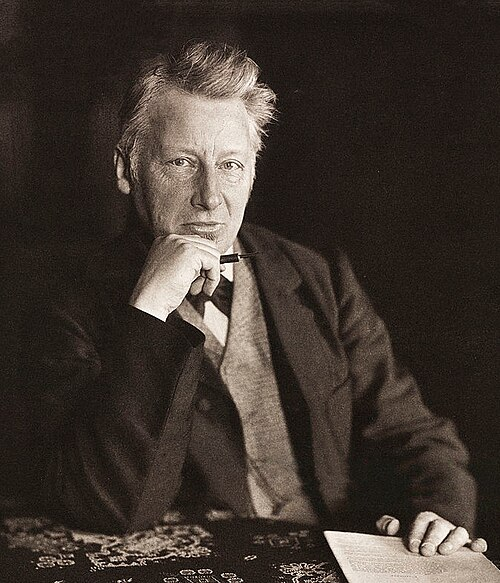
\includegraphics[width=\linewidth]{images/book3/vanthoff.jpg}
\end{minipage}\hfill
\begin{minipage}[t]{0.76\linewidth}\vspace{0pt}
ياكوبوس هنريكوس فانت هوف (1852--1911) أعطى سنة 1884، في كتابه
\emph{دراسات في الديناميكا الكيميائية}، العلاقة بين درجة الحرارة وثابت
التوازن التي تحمل اسمه، وفي السنة التالية قانون \omterm{def:b2:chemical-potential:osmotic-pressure}{الضغط الأسموزي} الوارد في
\cref{ch:b2:chemical-potential}؛ وكان قبل ذلك بعشر سنوات قد اقترح ذرة الكربون
الرباعية الأوجه. ونال أول جائزة نوبل في الكيمياء، سنة 1901. (صورة بعدسة
ن. پيرشايد، 1904: ملكية عامة،
ويكيميديا كومنز.)
\end{minipage}
\end{history}

\section{التغايرية}

كم مقدارًا مكثفًا يستطيع المجرّب أن يثبّته بحرية قبل أن تتحدد حالة
التوازن تمامًا؟

\begin{definition}[التغايرية]\label{def:b2:equilibrium-shifts:variance}
\emph{الوسائط المكثفة المستقلة}\index{وسيط مكثف مستقل}
لنظام في توازن هي مجموعة من المقادير المكثفة
(درجة الحرارة، والضغط، والكسور المولية في كل طور) يمكن اختيارها
مستقلةً، وإذا اختيرت ثبّتت كل المقادير الأخرى. وعددها هو
\emph{تغايرية}\index{تغايرية} النظام $v$.
\end{definition}

\begin{theorem}[قاعدة الأطوار]\label{thm:b2:equilibrium-shifts:phase-rule}
من أجل نظام من $n$ نوعًا كيميائيًا موزعة على $\varphi$ طورًا، ترتبط بعدد $r$
من التفاعلات المتوازنة المستقلة وبعدد $s$ من العلاقات الإضافية بين المقادير
المكثفة تفرضها طريقة التحضير (تغذية ستوكيومترية،
تعادل كهربائي)،
\[
  v = c + 2 - \varphi, \qquad c = n - r - s .
\]
\end{theorem}

\begin{proof}
المتغيرات المكثفة: $T$، و$p$، وفي كل طور الكسور المولية
للأنواع $n$، ومجموعها 1، فمنها $n - 1$ حرة في كل طور: فيكون المجموع $2 +
\varphi(n - 1)$. والعلاقات: كل نوع في توازن بين
الأطوار، أي $\varphi - 1$ مساواة بين الجهود الكيميائية لكل نوع، و$n(\varphi -
1)$ في المجموع؛ وكل تفاعل يعطي $Q = K^\circ(T)$، أي $r$ علاقة؛ و$s$
علاقة إضافية. وبالطرح: $v = 2 + \varphi(n - 1) - n(\varphi - 1) - r -
s = n - r - s + 2 - \varphi$. (وغياب نوع عن طور ما يحذف متغيرًا
وعلاقة معًا.)
\end{proof}

\begin{method}[حساب التغايرية]\label{met:b2:equilibrium-shifts:variance}
\begin{enumerate}
  \item اذكر الأنواع الكيميائية مع أطوارها، وعدّ $n$ و$\varphi$
        (كل جسم صلب نقي طور؛ والغازات كلها طور واحد).
  \item عدّ التفاعلات المستقلة $r$ بينها.
  \item عدّ العلاقات الإضافية $s$: كميات بنسب ستوكيومترية
        (فقط إذا كانت العلاقة بين مقادير في الطور نفسه)،
        والتعادل الكهربائي لمحلول أيوني.
  \item $v = n - r - s + 2 - \varphi$.
\end{enumerate}
\end{method}

\begin{example}[ثلاث تغايريات]\label{ex:b2:equilibrium-shifts:variances}
الحجر الجيري في وعاء مغلق، \ce{CaCO3(s) <=> CaO(s) + CO2(g)}: $n = 3$، $r =
1$، $\varphi = 3$ (جسمان صلبان، وغاز واحد): $v = 1$. اختر $T$، فيتحدد ضغط
ثنائي أكسيد الكربون: $p = K^\circ(T)\,p^\circ$. وخليط غازي من
\ce{N2} و\ce{H2} و\ce{NH3} في توازن: $n = 3$، $r = 1$، $\varphi = 1$، $v
= 3$ ($T$ و$p$ ومتغير تركيب واحد)؛ وإذا صُنع من الأمونيا وحدها، أو من
تغذية ستوكيومترية، كان \ce{N2} و\ce{H2} بالنسبة 1 : 3، و$s = 1$
و$v = 2$: فعند $T$ و$p$ معلومين يتحدد التركيب، كما تستعمل ذلك مسألة
نهاية الأسبوع.
\end{example}

\section{إزاحة التوازن}

\begin{definition}[انزياح التوازن]\label{def:b2:equilibrium-shifts:shift}
حين يُضطرب نظام في توازن (بتغيير درجة الحرارة، أو الضغط، أو كمية
مادة)، لا يبقى عمومًا في توازن ويتطور نحو توازن جديد. ويكون
\emph{انزياح التوازن}\index{انزياح التوازن}
في الاتجاه المباشر إذا تقدم التفاعل ($\dd\xi > 0$) وفي الاتجاه المعاكس
في غير ذلك.
\end{definition}

\begin{method}[التنبؤ بانزياح]\label{met:b2:equilibrium-shifts:predict-shift}
مباشرة بعد الاضطراب، احسب $Q$ و$K^\circ$ (أو قدّر إشارة تغيرهما). فإذا صار
$Q < K^\circ$، كان الانزياح في الاتجاه المباشر؛ وإذا صار $Q > K^\circ$،
ففي الاتجاه المعاكس؛ وإذا بقيت المساواة قائمة، فلا انزياح.
\end{method}

\begin{omfigure}
\begin{tikzpicture}[font=\small, >={Stealth}]
  \draw[->, thick] (0,0) -- (11,0) node[right] {$\ln Q$};
  \draw[omThm, thick] (5.5,0.25) -- (5.5,-0.25) node[below, align=center] {$\ln K^\circ$\\ \foreignlanguage{arabic}{قبلًا $= \ln Q$}};
  \fill (5.5,0) circle (2pt);
  \draw[omDef, thick] (2.8,0.25) -- (2.8,-0.25) node[below] {\foreignlanguage{arabic}{$\ln Q$ بُعيد الاضطراب}};
  \draw[->, omDef, very thick] (3.0,0.6) -- (5.2,0.6) node[midway, above] {انزياح مباشر};
  \draw[omProp, thick] (8.4,0.25) -- (8.4,-0.25) node[below] {\foreignlanguage{arabic}{$\ln Q$ بُعيد الاضطراب}};
  \draw[->, omProp, very thick] (8.2,0.6) -- (5.8,0.6) node[midway, above] {انزياح معاكس};
\end{tikzpicture}

{\small يحرّك الاضطرابُ $Q$ (أو $K^\circ$ إذا تغيرت درجة الحرارة)؛
ثم ينزاح النظام حتى يعود $Q = K^\circ$، في الاتجاه المباشر إذا صار $Q$
صغيرًا جدًا، وفي الاتجاه المعاكس إذا صار كبيرًا جدًا.}
\end{omfigure}

\begin{proposition}[درجة الحرارة]\label{prop:b2:equilibrium-shifts:temperature}
عند ضغط ثابت، يزيح رفعُ درجة الحرارة التوازنَ في الاتجاه
\omterm{def:b2:reaction-enthalpy:exothermic}{الماص للحرارة} (المباشر إذا كان $\Delta_r H^\circ > 0$)، ويزيحه خفضُها في
الاتجاه \omterm{def:b2:reaction-enthalpy:exothermic}{الناشر للحرارة}.
\end{proposition}

\begin{proof}
عند تركيب وضغط ثابتين، لا يتغير $Q$ مع $T$ (في الأنظمة
المثالية)؛ وحسب فانت هوف، يزداد $K^\circ$ مع $T$ إذا كان $\Delta_r H^\circ >
0$. فمباشرة بعد ارتفاع $T$ يكون إذن $Q < K^\circ$: في الاتجاه المباشر.
\end{proof}

\begin{proposition}[الضغط]\label{prop:b2:equilibrium-shifts:pressure}
عند درجة حرارة وتركيب ثابتين، يزيح رفعُ الضغط الكلي لتوازن في الطور
الغازي هذا التوازنَ في الاتجاه الذي يقلل عدد الجزيئات
الغازية (المباشر إذا كان $\Delta\nu_{\text{غاز}} < 0$). وإذا كان $\Delta\nu_{\text{غاز}}
= 0$، فلا أثر للضغط.
\end{proposition}

\begin{proof}
مع $p_i = x_ip$، يكون $Q = \prod_i x_i^{\nu_i}\,(p/p^\circ)^{\Delta\nu_{\text{غاز}}}$:
فعند تركيب ثابت، يضرب رفعُ $p$ المقدارَ $Q$ في
$(p'/p)^{\Delta\nu_{\text{غاز}}}$، وهو $< 1$ إذا كان $\Delta\nu_{\text{غاز}} <
0$. فيكون $Q < K^\circ$: في الاتجاه المباشر. والأطوار المكثفة لا تساهم بشيء.
\end{proof}

\begin{proposition}[إضافة مكوّن أو غاز خامل]\label{prop:b2:equilibrium-shifts:adding}
إضافة كمية صغيرة من مكوّن غازي $j$ إلى توازن في الطور الغازي
تغيّر $\ln Q$ بمقدار
\[
  \left(\frac{\partial\ln Q}{\partial n_j}\right) = \frac{\nu_j}{n_j} -
  \frac{\Delta\nu_{\text{غاز}}}{n_{\text{كلي}}}\ \ \text{عند ثبات } T, p ;
  \qquad \frac{\nu_j}{n_j}\ \ \text{عند ثبات } T, V .
\]
إضافة غاز خامل لا أثر لها عند حجم ثابت، وتؤثر عند ضغط ثابت
تأثير خفض الضغط.
\end{proposition}

\begin{proof}
عند $T$ و$p$ ثابتين: $Q = \prod_i n_i^{\nu_i}\,(p/(p^\circ n_{\text{كلي}}))^{
\Delta\nu_{\text{غاز}}}$، ومشتقته اللوغاريتمية بالنسبة إلى $n_j$ هي
$\nu_j/n_j - \Delta\nu_{\text{غاز}}/n_{\text{كلي}}$ (الحد الأول منعدم لغاز
خامل، $\nu_j = 0$). وعند $T$ و$V$ ثابتين: $p_i = n_iRT/V$ و$Q = \prod_i n_i^{
\nu_i}\,(RT/(p^\circ V))^{\Delta\nu_{\text{غاز}}}$، ومشتقته
$\nu_j/n_j$ وحدها.
\end{proof}

\begin{remark}[متفاعل يُضاف فيدفع التفاعل في الاتجاه المعاكس]\label{rem:b2:equilibrium-shifts:paradox}
في تخليق الأمونيا، $\nu(\ce{N2}) = -1$ و$\Delta\nu_{\text{غاز}} = -2$:
فإضافة النيتروجين عند $T$ و$p$ ثابتين تغيّر $\ln Q$ بمقدار $-1/n_{\ce{N2}} +
2/n_{\text{كلي}}$، وهو موجب حين يكون $x(\ce{N2}) > 1/2$. ففي خليط
غني أصلًا بالنيتروجين، تخفف إضافة مزيد من النيتروجين الهيدروجينَ إلى حد
تتفكك معه الأمونيا. فالقاعدة «إضافة متفاعل تدفع في الاتجاه المباشر» آمنة
عند حجم ثابت، لا دائمًا عند ضغط ثابت.
\end{remark}

\begin{proposition}[مبدأ لوشاتلييه]\label{prop:b2:equilibrium-shifts:le-chatelier}
تُلخَّص القضايا السابقة في \emph{مبدأ
لوشاتلييه}\index{مبدأ لوشاتلييه}: النظام في توازن،
إذا اضطرب في درجة حرارته أو ضغطه، ينزاح في الاتجاه الذي يعاكس
الاضطراب (فيمتص الحرارة إذا سُخّن، ويقلل حجمه الغازي إذا
ضُغط).
\end{proposition}

\begin{proof}
إنه إعادة صياغة \cref{prop:b2:equilibrium-shifts:temperature} (فالاتجاه
\omterm{def:b2:reaction-enthalpy:exothermic}{الماص للحرارة} يمتص الحرارة) و\cref{prop:b2:equilibrium-shifts:pressure} (فالجزيئات
الغازية الأقل عددًا تشغل حجمًا أصغر عند $T$ و$p$ نفسيهما). أما في إضافات
المادة عند ضغط ثابت فالمبدأ غير موثوق
(\cref{rem:b2:equilibrium-shifts:paradox}): احسب $Q$.
\end{proof}

\begin{remark}[حين ينتهي التوازن]\label{rem:b2:equilibrium-shifts:rupture}
قد لا ينتهي الانزياح إلى توازن جديد بل إلى اختفاء طور.
فالحجر الجيري المسخَّن في وعاء مغلق يتفكك حتى يصير $p(\ce{CO2}) =
K^\circ(T)\,p^\circ$؛ فإن لم تكفِ كميته لبلوغ ذلك الضغط،
اختفى كليًا وبقي $Q$ أدنى من $K^\circ$: فيخرج النظام من
التوازن نهائيًا، كما لاحظ ذلك مجلد السنة الأولى.
\end{remark}

\begin{history}[هنري لوشاتلييه]
\begin{minipage}[t]{0.2\linewidth}\vspace{0pt}
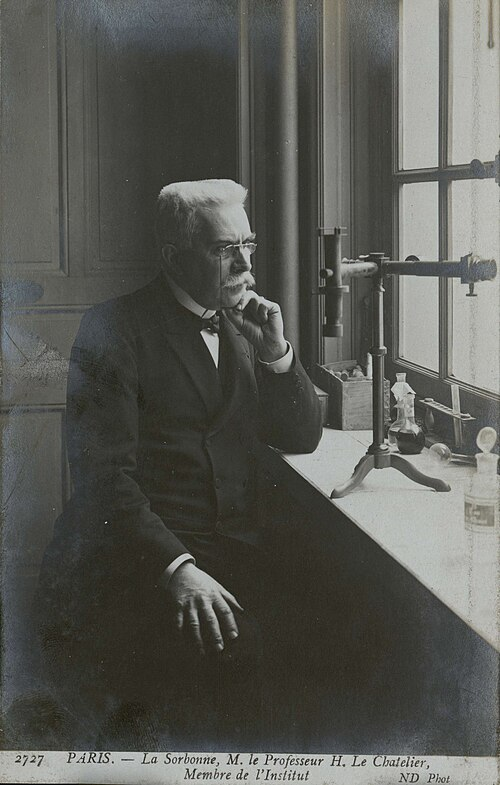
\includegraphics[width=\linewidth]{images/book3/lechatelier.jpg}
\end{minipage}\hfill
\begin{minipage}[t]{0.76\linewidth}\vspace{0pt}
هنري لوشاتلييه (1850--1936)، مهندس مناجم وكيميائي عمل على
الإسمنت والتعدين وقياس درجات الحرارة العالية، صاغ سنة 1884 «قانون \omterm{def:b2:equilibrium-shifts:shift}{انزياح
التوازن}» الذي يحمل اسمه. وكان قد حاول أيضًا، نحو سنة 1901، صنع
الأمونيا من عنصريها تحت الضغط؛ فأنهى انفجارٌ في جهازه
المحاولة. (صورة: مؤلف مجهول، CC~BY-SA~4.0، ويكيميديا كومنز.)
\end{minipage}
\end{history}

\section{تحسين تخليق}

\subsection*{الأمونيا}

\begin{omfigure}
\begin{tikzpicture}
\begin{axis}[
  width=0.78\linewidth, height=6.2cm, xmin=500, xmax=1000, ymin=0, ymax=0.9,
  axis x line=bottom, axis y line=left, xlabel={\babelsublr{$T$ (K)}},
  ylabel={\foreignlanguage{arabic}{الكسر المولي للأمونيا \ce{NH3} عند التوازن}},
  tick label style={font=\small}, label style={font=\small}, clip=false]
\addplot[omThm, very thick] table[x=T, y=p300] {figdata/out/bachelor-2-vant-hoff-b.dat};
\addplot[omDef, very thick] table[x=T, y=p200] {figdata/out/bachelor-2-vant-hoff-b.dat};
\addplot[omProp, very thick] table[x=T, y=p50] {figdata/out/bachelor-2-vant-hoff-b.dat};
\addplot[black!60, very thick] table[x=T, y=p1] {figdata/out/bachelor-2-vant-hoff-b.dat};
\node[omThm, font=\scriptsize, anchor=south west] at (axis cs:600,0.70) {\qty{300}{bar}};
\node[omDef, font=\scriptsize, anchor=north east] at (axis cs:612,0.52) {\qty{200}{bar}};
\node[omProp, font=\scriptsize, anchor=north east] at (axis cs:578,0.30) {\qty{50}{bar}};
\node[black!60, font=\scriptsize, anchor=south west] (onebar) at (axis cs:520,0.13) {\qty{1}{bar}};
\draw[black!60] (onebar.south west) -- (axis cs:512,0.075);
\draw[dotted] (axis cs:723,0) -- (axis cs:723,0.253);
\fill[omDef] (axis cs:723,0.253) circle (1.6pt);
\end{axis}
\end{tikzpicture}

{\small الكسر المولي للأمونيا عند التوازن انطلاقًا من خليط 1 : 3 من النيتروجين
والهيدروجين (غازات مثالية)، بدلالة درجة الحرارة عند أربعة ضغوط،
محسوبًا من طاقات جيبس المجدولة. الضغط يرفعه، ودرجة الحرارة
تخفضه؛ والنقطة تشير إلى \qty{723}{K} و\qty{200}{bar}.}
% ledger: janafG:NH3.500, janafG:NH3.600, janafG:NH3.700, janafG:NH3.800, janafG:NH3.900, janafG:NH3.1000 (computed in figdata/bachelor-2/vant-hoff.py)
\end{omfigure}

التخليق \omterm{def:b2:reaction-enthalpy:exothermic}{ناشر للحرارة} ويحوّل أربعة جزيئات غازية إلى جزيئين: فحسب
القضايا السابقة، تحابي درجة الحرارة المنخفضة والضغط المرتفع الأمونيا.
وعند \qty{1}{bar} ودرجة حرارة الغرفة يكاد التوازن يكون تامًا، لكن
التفاعل لا يجري إطلاقًا: فالرابطة الثلاثية للنيتروجين لا تُكسر إلا
على حفاز، وحفاز الحديد لا يعمل إلا عند عدة مئات من
الدرجات. ولهذا تختار المصانع:
\begin{itemize}
  \item درجة حرارة عالية بما يكفي للسرعة، ومنخفضة بقدر ما يسمح الحفاز
        (نحو \qty{700}{K})؛
  \item ضغطًا مرتفعًا لاسترجاع المردود الذي تُفقده درجة الحرارة، تحدّه
        كلفة الضغط وكلفة الأوعية السميكة الجدران؛
  \item حلقة: يُبرَّد الغاز الخارج من المحوِّل، فتتكثف الأمونيا
        وتُنزع، ويُعاد تدوير الغاز غير المحوَّل مع التغذية الطازجة؛
        ويزيل \omterm{def:b2:equilibrium-shifts:single-pass}{تنفيس} صغير الأرغون والميثان اللذين كانا سيتراكمان
        لولاه.
\end{itemize}

\begin{definition}[التحويل في مرور واحد، إعادة التدوير، التنفيس]\label{def:b2:equilibrium-shifts:single-pass}
في عملية بإعادة تدوير، يكون \emph{التحويل في مرور واحد}\index{تحويل في مرور واحد}
هو كسر المتفاعل المحوَّل في مرور واحد عبر
المفاعل؛ والجزء غير المحوَّل، بعد فصله عن الناتج، يُعاد إلى مدخل المفاعل
ويُسمّى \emph{تيار إعادة التدوير}\index{تيار إعادة التدوير}؛ و\emph{التنفيس}\index{تنفيس}
تيار صغير يُسحب باستمرار من تيار إعادة التدوير لمنع تراكم الأنواع
الخاملة.
\end{definition}

\begin{omfigure}
\begin{tikzpicture}[font=\small, >={Stealth}, box/.style={draw, thick, rounded corners=2pt, minimum width=2.1cm, minimum height=1.0cm, align=center, fill=white}]
  \node[box] (comp) at (0,0) {ضاغط};
  \node[box] (conv) at (3.6,0) {\shortstack{\foreignlanguage{arabic}{المحوِّل}\\\foreignlanguage{arabic}{(الحفاز)}}};
  \node[box] (cond) at (7.2,0) {مبرِّد\\ وفاصل};
  \draw[->, thick] (-3.9,0) -- (comp) node[pos=0.0, above right] {\foreignlanguage{arabic}{\ce{N2 + 3H2} طازج}};
  \draw[->, thick] (comp) -- (conv);
  \draw[->, thick] (conv) -- (cond);
  \draw[->, thick, omDef] (cond.south) -- ++(0,-1.0) node[below] {أمونيا سائلة};
  \draw[->, thick, omThm] (cond.north) -- ++(0,0.9) -| (comp.north);
  \node[omThm, above] at (2.6,1.4) {\shortstack{\foreignlanguage{arabic}{إعادة التدوير (الغاز غير المحوَّل)}}};
  \draw[->, thick, black!60] (6.1,1.4) -- (6.1,2.1) node[above] {تنفيس};
\end{tikzpicture}

{\small حلقة الأمونيا. كل مرور لا يحوّل إلا جزءًا من الغاز؛ فتُكثَّف الأمونيا
وتُفصل، ويُعاد ضغط الباقي ويُرسل ثانية مع التغذية
الطازجة. ويمنع \omterm{def:b2:equilibrium-shifts:single-pass}{التنفيس} الأرغون والميثان، اللذين لا يتفاعلان، من
التراكم.}
\end{omfigure}

\begin{history}[هابر وبوش]
\begin{minipage}[t]{0.15\linewidth}\vspace{0pt}
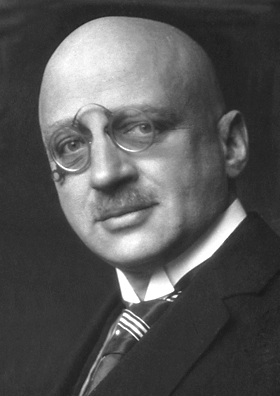
\includegraphics[width=\linewidth]{images/book3/haber.png}
\end{minipage}\hspace{0.01\linewidth}%
\begin{minipage}[t]{0.15\linewidth}\vspace{0pt}
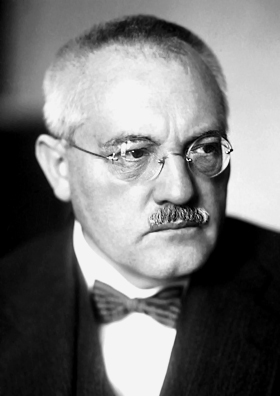
\includegraphics[width=\linewidth]{images/book3/bosch.jpg}
\end{minipage}\hfill
\begin{minipage}[t]{0.66\linewidth}\vspace{0pt}
قاس فريتز هابر (1868--1934) توازن الأمونيا تحت الضغط،
وجعلها سنة 1909 تتدفق باستمرار من محوِّل مخبري فوق حفاز من
الأوزميوم. وحوّل كارل بوش (1874--1940) ذلك إلى صناعة، بأوعية من
الفولاذ تقاوم الهيدروجين الساخن تحت الضغط وبحفاز رخيص من الحديد؛
وبدأ أول مصنع العمل سنة 1913. ونال هابر جائزة نوبل سنة
1918، وبوش سنة 1931. (صور مؤسسة نوبل: ملكية عامة، ويكيميديا كومنز.)
\end{minipage}
\end{history}

\subsection*{ثالث أكسيد الكبريت}

في عملية التلامس يجري التفاعل \ce{2SO2(g) + O2(g) <=> 2SO3(g)} ($\Delta_r H^\circ =
\qty{-197.8}{kJ/mol}$ للمعادلة كما هي مكتوبة) على حفاز من أكسيد
الفاناديوم لا ينشط إلا ساخنًا، في عدة طبقات كظومة. في كل طبقة ترفع الحرارة
المحررة درجة الحرارة، وهو ما يخفض $K^\circ$؛ فيتوقف التحويل حين يبلغ الغاز
منحنى التوازن. والتبريد بين الطبقات يعيده إلى درجة حرارة يسمح عندها
التوازن بمزيد من التحويل.
% ledger: dfh:SO2_g, dfh:SO3_g

\begin{omfigure}
\begin{tikzpicture}
\begin{axis}[
  width=0.72\linewidth, height=6.4cm, xmin=600, xmax=900, ymin=0, ymax=1.08,
  axis x line=bottom, axis y line=left, xlabel={\babelsublr{$T$ (K)}},
  ylabel={\foreignlanguage{arabic}{تحويل \ce{SO2}}}, tick label style={font=\small},
  label style={font=\small}, clip=false]
\addplot[black, very thick] table[x=T, y=X] {figdata/out/bachelor-2-vant-hoff-c.dat};
\addplot[omThm, thick] table[x=T, y=X] {figdata/out/bachelor-2-vant-hoff-bed1.dat};
\addplot[omThm, thick] table[x=T, y=X] {figdata/out/bachelor-2-vant-hoff-bed2.dat};
\addplot[omThm, thick] table[x=T, y=X] {figdata/out/bachelor-2-vant-hoff-bed3.dat};
\draw[->, omDef, thick] (axis cs:892.8,0.676) -- (axis cs:712,0.676);
\draw[->, omDef, thick] (axis cs:784.4,0.924) -- (axis cs:712,0.924);
\node[font=\scriptsize, anchor=south west] at (axis cs:860,0.84) {التوازن};
\node[omThm, font=\scriptsize, anchor=west] at (axis cs:800,0.24) {\shortstack{\foreignlanguage{arabic}{الطبقة \babelsublr{1} (كظومة)}}};
\node[omDef, font=\scriptsize, anchor=south] at (axis cs:800,0.68) {تبريد};
\end{axis}
\end{tikzpicture}

{\small التحويل عند التوازن لثنائي أكسيد الكبريت \ce{SO2} إلى \ce{SO3} بدلالة درجة الحرارة
(بالأسود) لتغذية نموذجية فيها \qty{10}{\percent} من \ce{SO2} و\qty{11}{\percent}
من \ce{O2} عند \qty{1}{bar}، ومسار الغاز عبر ثلاث طبقات كظومة
(بالأحمر، ترتفع درجة حرارته إذ يسخّن التفاعل الغاز)، مع التبريد بين
الطبقات (بالأزرق).}
% ledger: janafG:SO2.600, janafG:SO2.700, janafG:SO2.800, janafG:SO2.900, janafG:SO3.600, janafG:SO3.700, janafG:SO3.800, janafG:SO3.900 (computed in figdata/bachelor-2/vant-hoff.py; feed and adiabatic rise are model values)
\end{omfigure}

\section{تمارين}

\begin{exercise}[$\star$]\label{exo:b2:equilibrium-shifts:1}
احسب $K^\circ$ عند \qty{298}{K} لتفاعل فيه $\Delta_r G^\circ =
\qty{-32.8}{kJ/mol}$، ثم من أجل $\Delta_r G^\circ = \qty{+32.8}{kJ/mol}$.
ما تغيّر $\Delta_r G^\circ$ الذي يضرب $K^\circ$ في 100؟
\end{exercise}

\begin{exercise}[$\star$]\label{exo:b2:equilibrium-shifts:2}
من أجل تخليق الأمونيا $K^\circ(298) = \num{5.4e5}$ و$\Delta_r H^\circ =
\qty{-91.9}{kJ/mol}$. قدّر $K^\circ$ عند \qty{400}{K} \omterm{thm:b2:equilibrium-shifts:vant-hoff}{بمعادلة فانت هوف}
المكاملة؛ والجداول تعطي 35.6.
\end{exercise}

\begin{exercise}[$\star$]\label{exo:b2:equilibrium-shifts:3}
احسب \omterm{def:b2:equilibrium-shifts:variance}{تغايرية}: (أ) الماء السائل في توازن مع بخاره؛
(ب) \ce{CaCO3(s) <=> CaO(s) + CO2(g)} في وعاء مغلق؛ (ج) \ce{N2}
و\ce{H2} و\ce{NH3} في توازن، بتغذية كيفية؛ (د) \ce{C(s) + H2O(g) <=>
CO(g) + H2(g)}.
\end{exercise}

\begin{exercise}[$\star$]\label{exo:b2:equilibrium-shifts:4}
من أجل \ce{N2O4(g) <=> 2NO2(g)}، $\Delta_r H^\circ > 0$. في أي اتجاه
ينزاح التوازن بالتسخين عند ضغط ثابت، وبالضغط عند درجة حرارة
ثابتة، وبإضافة الأرغون عند حجم ثابت؟
\end{exercise}

\begin{exercise}[$\star\star$]\label{exo:b2:equilibrium-shifts:5}
من أجل \ce{N2(g) + O2(g) <=> 2NO(g)}، $\Delta_r H^\circ = \qty{180.6}{kJ/mol}$،
$\Delta_r S^\circ = \qty{24.8}{J/(K.mol)}$. احسب $K^\circ$ عند \qty{298}{K}
وعند \qty{2000}{K} (\omterm{def:b2:reaction-free-energy:ellingham-approximation}{تقريب إلينغهام})، والكسر المولي لأحادي أكسيد النيتروجين
\ce{NO} في الهواء ($x(\ce{N2}) = 0.78$، $x(\ce{O2}) = 0.21$، قليلًا ما يُستهلكان) عند
التوازن عند \qty{2000}{K}. لماذا تصنع المحركات هذا الملوِّث، ولماذا
يبقى في غازات العادم المبرَّدة؟
\end{exercise}

\begin{exercise}[$\star\star$]\label{exo:b2:equilibrium-shifts:6}
لتفاعل أسترة $\mathrm{A + B \rightleftharpoons E + W}$ في الطور السائل
ثابت $K^\circ = 4.0$ (مع أخذ النشاطيات كسورًا مولية). انطلاقًا من
\qty{1.0}{mol} من الحمض A، احسب كمية الإستر مع \qty{1.0}{mol}، ثم مع
\qty{3.0}{mol} من الكحول B. وفسّر، بواسطة $Q$ و$K^\circ$، لماذا يدفع نزعُ
الماء كلما تكوّن التفاعلَ حتى نهايته.
\end{exercise}

\begin{exercise}[$\star\star$]\label{exo:b2:equilibrium-shifts:7}
عند \qty{298}{K} و\qty{1}{bar}، $K^\circ = 0.148$ للتفاعل \ce{N2O4 <=> 2NO2}.
احسب درجة تفكك \qty{1}{mol} من \ce{N2O4}. ثم يُضاف
\qty{1}{mol} من الأرغون عند ضغط كلي ثابت: احسب درجة
التفكك الجديدة، وفسّر. ماذا يحدث إذا أُضيف الأرغون عند
حجم ثابت؟
\end{exercise}

\begin{exercise}[$\star\star$]\label{exo:b2:equilibrium-shifts:8}
يتسامى كلوريد الأمونيوم بالتفكك، \ce{NH4Cl(s) <=> NH3(g) +
HCl(g)}. احسب \omterm{def:b2:equilibrium-shifts:variance}{التغايرية} حين لا يصنع الغازَ إلا الجسمُ الصلب، وحين
تُضاف بعض الأمونيا. ماذا تعني كل حالة بالنسبة إلى المجرّب؟
\end{exercise}

\begin{exercise}[$\star\star$]\label{exo:b2:equilibrium-shifts:9}
تعطي الجداول، لتخليق الأمونيا، $K^\circ = 0.0993$ عند \qty{500}{K} 
و$K^\circ = \num{1.72e-3}$ عند \qty{600}{K}. استنتج $\Delta_r H^\circ$ في هذه
الفترة وقارنه بقيمته عند \qty{298}{K}.
\end{exercise}

\begin{exercise}[$\star\star\star$]\label{exo:b2:equilibrium-shifts:10}
برهن المثال المضاد في \cref{rem:b2:equilibrium-shifts:paradox}: اكتب
$Q$ لتخليق الأمونيا بدلالة كميات المادة والضغط الكلي، واحسب
$\partial\ln Q/\partial n(\ce{N2})$ عند $T$ و$p$ ثابتين، وأوجد
الشرط على $x(\ce{N2})$ الذي تزيح عنده إضافة النيتروجين التوازن في الاتجاه
المعاكس. هل يمكن أن يحدث الشيء نفسه عند حجم ثابت؟
\end{exercise}

\begin{exercise}[$\star\star\star$]\label{exo:b2:equilibrium-shifts:11}
يُسخَّن الحجر الجيري إلى \qty{1100}{K} في وعاء مغلق فارغ حجمه
\qty{10.0}{L}، حيث $\Delta_r G^\circ = \qty{1.62}{kJ/mol}$ لتفككه
(\cref{ch:b2:reaction-free-energy}). احسب $K^\circ$ وضغط التوازن لثنائي
أكسيد الكربون. وأوجد الحالة النهائية من أجل
\qty{0.050}{mol} ومن أجل \qty{0.200}{mol} من الحجر الجيري.
\end{exercise}

\begin{exercise}[$\star\star\star$]\label{exo:b2:equilibrium-shifts:12}
اقرأ على شكل عملية التلامس التحويلَ ودرجة الحرارة عند مخرج كل
طبقة. وفسّر لماذا لا تستطيع طبقة كظومة واحدة، مهما طالت، أن تتجاوز نحو
68\,\% من التحويل بهذه التغذية، ولماذا يُبرَّد الغاز بين الطبقات بدل إبقاء
الحفاز باردًا طوال الوقت، وما الذي يحدّ تحويل الطبقة الأخيرة.
\end{exercise}

\section{مسألة: حلقة الأمونيا}

\begin{problem}[{مسألة نهاية الأسبوع --- ثابت توازن تخليق الأمونيا وتعلقه
بدرجة الحرارة، والتركيب في شروط المحوِّل، والانزياحات التي يسببها الضغط
ودرجة الحرارة والغازات الخاملة، والحلقة}]
\label{pb:b2:equilibrium-shifts:1}
تُصنع الأمونيا وفق \ce{N2(g) + 3H2(g) <=> 2NH3(g)} من تغذية ستوكيومترية.
المعطيات: عند \qty{298.15}{K}، $\Delta_f H^\circ(\ce{NH3}) = \qty{-45.94}{kJ/mol}$،
و$S^\circ_m$ (\unit{J/(K.mol)}) \ce{NH3} 192.77، \ce{N2} 191.61، \ce{H2} 130.68؛
وتعطي الجداول $\Delta_f G^\circ(\ce{NH3}) = \qty{+27.19}{kJ/mol}$ عند
\qty{700}{K} و\qty{+38.66}{kJ/mol} عند \qty{800}{K}. الغازات مثالية؛
$R = \qty{8.314}{J/(K.mol)}$.
% ledger: dfh:NH3_g, s0:NH3_g, s0:N2_g, s0:H2_g, janafG:NH3.700, janafG:NH3.800

\medskip
\noindent\textbf{الجزء الأول --- الثابت.}
\begin{enumerate}
  \item احسب $\Delta_r H^\circ$ و$\Delta_r S^\circ$ و$\Delta_r G^\circ$ عند
        \qty{298}{K}، و$K^\circ(298)$.
  \item احسب $K^\circ$ عند \qty{700}{K} وعند \qty{800}{K} من الجداول.
  \item استنتج من هاتين القيمتين متوسط $\Delta_r H^\circ$ بين
        \qty{700}{K} و\qty{800}{K}، وقارنه بالسؤال 1.
  \item قدّر $K^\circ(\qty{723}{K})$ من القيمتين المجدولتين بواسطة
        \omterm{thm:b2:equilibrium-shifts:vant-hoff}{معادلة فانت هوف}.
  \item احسب $K^\circ(\qty{723}{K})$ في \omterm{def:b2:reaction-free-energy:ellingham-approximation}{تقريب إلينغهام} انطلاقًا من
        المعطيات عند \qty{298}{K}، وعلّق على الفرق.
\end{enumerate}

\medskip
\noindent\textbf{الجزء الثاني --- التوازن في المحوِّل.}
\begin{enumerate}[resume]
  \item انطلاقًا من تغذية من \qty{1}{mol} من \ce{N2} و\qty{3}{mol} من \ce{H2}، اكتب
        كميات المادة عند التقدم $\xi$ وكمية المادة الكلية.
  \item بيّن أنه، إذا كان $x$ الكسر المولي للأمونيا، فإن الكسرين الموليين
        للنيتروجين \ce{N2} والهيدروجين \ce{H2} هما $(1-x)/4$ و$3(1-x)/4$.
  \item بيّن أن $\dfrac{x}{(1-x)^2} = \dfrac{\sqrt{27}}{16}\,\dfrac{p}{p^\circ}\,
        \sqrt{K^\circ}$.
  \item احسب $x$ عند \qty{723}{K} و\qty{1}{bar}.
  \item احسب $x$ عند \qty{723}{K} و\qty{200}{bar}.
  \item احسب \omterm{def:b2:equilibrium-shifts:variance}{تغايرية} النظام وفسّر لماذا يحدد $T$ و$p$
        التركيب.
\end{enumerate}

\medskip
\noindent\textbf{الجزء الثالث --- الانزياحات.}
\begin{enumerate}[resume]
  \item دون حساب، في أي اتجاه ينزاح التوازن حين يرتفع
        الضغط؟ وحين ترتفع درجة الحرارة؟
  \item يدخل الأرغون مع الهواء المستعمل في تحضير النيتروجين. كيف يزيح وجوده
        التوازن عند ضغط كلي ثابت؟
  \item لخليط في توازن $x(\ce{N2}) = 0.30$. هل تزيحه إضافة قليل من
        النيتروجين عند $T$ و$p$ ثابتين في الاتجاه المباشر أم في الاتجاه المعاكس؟
  \item هل يتغير الجواب عند حجم ثابت؟
  \item قبل أن يعود الغاز إلى المحوِّل، تُكثَّف أمونياه
        وتُنزع. ماذا يفعل ذلك بالمقدار $Q$ عند مدخل المحوِّل؟
\end{enumerate}

\medskip
\noindent\textbf{الجزء الرابع --- الحلقة.}
\begin{enumerate}[resume]
  \item يغادر الغاز المحوِّلَ وفيه \qty{18}{\percent} من الأمونيا، أي أقل من
        قيمة التوازن. لماذا لا يبلغ المحوِّل الحقيقي
        التوازن؟
  \item احسب \omterm{def:b2:equilibrium-shifts:single-pass}{التحويل في مرور واحد} للهيدروجين الموافق
        للقيمة $x(\ce{NH3}) = 0.18$ انطلاقًا من تغذية ستوكيومترية.
  \item يُعاد تدوير الغاز غير المحوَّل. في التشغيل المستقر يدخل \qty{1.00}{mol}
        من \ce{N2} الطازج في وحدة الزمن: ما كمية الأمونيا الخارجة، وما
        كمية النيتروجين التي تعبر المحوِّل في وحدة الزمن؟
  \item لماذا يجب \omterm{def:b2:equilibrium-shifts:single-pass}{تنفيس} قليل من الغاز من \omterm{def:b2:equilibrium-shifts:single-pass}{تيار إعادة التدوير}؟
  \item لماذا لا يُشغَّل المحوِّل عند \qty{500}{K}، حيث التوازن
        أنسب بكثير؟
  \item اذكر الكسر المولي للأمونيا عند التوازن عند \qty{723}{K} 
        و\qty{200}{bar} لتغذية ستوكيومترية، في نموذج الغاز المثالي.
\end{enumerate}
\end{problem}
